\section{Problem (9)}
	A ball is shot vertically upward from the surface of another planet. A plot of $y$ versus $t$ for the ball is shown in \cref{fig:hw2_problem9},

	\begin{figure}[H]
		\begin{center}
			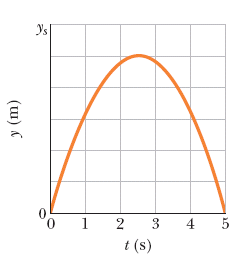
\includegraphics[scale=1]{hw2_problem9}
			\caption{Plot of $y$ versus $t$}
			\label{fig:hw2_problem9}
		\end{center}
	\end{figure}

	where $y$ is the height of the ball above its starting point and $t = 0$ at the instant the ball is shot. The point marked as $y_{s}$ has a value of $48.0 \ m$.

	\subsection{Question (a)}
		What is the magnitude of the free-fall acceleration on the planet?

		\textbf{R:} \newline

	\subsection{Question (b)}
		What is the magnitude of the initial velocity of the ball?

		\textbf{R:} \newline
